\section{微积分基本定理}
\label{sec:integ-ftc}

卷一的微积分基本定理有两个方向。被积函数$g$连续时，累计函数$G(x)=\int_a^xg(t)\,\mathrm dt$可导且$G'=g$；$F$连续可导时，$F(b)-F(a)=\int_a^bF'(t)\,\mathrm dt$。

有了Lebesgue积分，被积函数只需可积，导数也只需几乎处处存在，两个方向都要重新回答：可积函数的累计函数在什么意义下可导，导数是否回到被积函数？哪些函数能由几乎处处导数的积分恢复？本节在有界闭区间$[a,b]$上回答这两个问题，测度都是Lebesgue测度。

\subsection{变上限积分的导数}
\label{sec:integ-indefinite-derivative}

\paragraph{绝对连续函数}
先看什么样的函数有希望写成某个函数的累计。一致连续要求：区间足够短时，函数在两端的增量就小。要由导数恢复增量，这还不够。导数为零的点之间可能散布着许多极短的区间，函数恰好在这些区间上完成全部增长。需要控制的是许多互不相交的小区间上的\emph{总}增量。

\begin{definition}[绝对连续函数]
\label{def:integ-absolutely-continuous}
设$F:[a,b]\to\mathbb R$。若对任意$\varepsilon>0$存在$\delta>0$，使对$[a,b]$中任意有限个两两不交的开区间$(a_i,b_i)$（$i=1,\dots,m$），只要总长满足
\begin{equation}
 \sum_{i=1}^m(b_i-a_i)<\delta,
 \label{eq:integ-ac-length}
\end{equation}
就有
\begin{equation}
 \sum_{i=1}^m\lvert F(b_i)-F(a_i)\rvert<\varepsilon,
 \label{eq:integ-ac-increment}
\end{equation}
则称$F$为$[a,b]$上的\term{绝对连续函数}（absolutely continuous function）。
\end{definition}

取$m=1$就回到一致连续，所以绝对连续函数一致连续。区别在于$\delta$必须对任意多个小区间同时有效：区间个数不受限制，只限制总长度。图~\ref{fig:integ-absolute-continuity-intervals}中$F(x)=\sqrt x$，四段绿色区间总长$1.2$，对应的增量为
\[
 0.260,\qquad0.158,\qquad0.090,\qquad0.053,
\]
和约为$0.562$。绝对连续性要求，当总长趋于零时，增量之和也一致地趋于零，无论区间怎样分布、分成多少段。

\begin{BookInlineFigure}
  \centering
  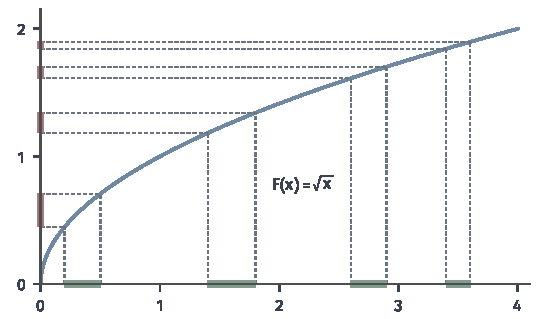
\includegraphics[width=92mm]{figures/04-spaces-measures-and-geometry/02-measure/matplotlib/integ-absolute-continuity-intervals/figure.pdf}
  \caption{绝对连续性控制的是多个不交区间上的总增量。$F(x)=\sqrt x$（蓝）。横轴上的绿色区间为$(0.2,0.5)$、$(1.4,1.8)$、$(2.6,2.9)$、$(3.4,3.6)$，纵轴上的红色线段是相应增量。靠近原点的区间虽短，增量却最大。}
  \label{fig:integ-absolute-continuity-intervals}
\end{BookInlineFigure}

若$F$满足Lipschitz条件$\lvert F(x)-F(y)\rvert\leq L\lvert x-y\rvert$，则总增量不超过$L$乘以总长度，取$\delta=\varepsilon/L$即可，所以Lipschitz函数绝对连续。$[a,b]$上连续可导的函数由中值定理满足Lipschitz条件，因而绝对连续。有限线性组合保持绝对连续，由三角不等式对各函数分别取$\delta$再取最小值即得。

这里的“绝对连续”描述函数增量受区间长度控制，与第~\ref{chap:measure-densities}章两个测度之间的绝对连续是不同的定义，两者的联系在那里说明。

\paragraph{变上限积分的绝对连续性}
设$g$在$[a,b]$上可积，令
\begin{equation}
 G(x)=\int_a^xg(t)\,\mathrm dt,\qquad a\leq x\leq b,
 \label{eq:integ-indefinite}
\end{equation}
称为$g$的\term{变上限积分}（indefinite integral）。多个不交区间上$G$的增量之和不超过$\lvert g\rvert$在这些区间之并上的积分，所以要证$G$绝对连续，需要的是：测度很小的集合上，$\lvert g\rvert$的积分也很小。

\begin{lemma}[积分的绝对连续性]
\label{lem:integ-small-sets}
设$g$关于$\mu$可积。则对任意$\varepsilon>0$存在$\delta>0$，使对每个满足$\mu(A)<\delta$的可测集$A$，都有$\int_A\lvert g\rvert\,\mathrm d\mu<\varepsilon$。
\end{lemma}

\begin{proof}
把$\lvert g\rvert$分成有界的截断$\min\{\lvert g\rvert,n\}$与尾部。截断随$n$递增到$\lvert g\rvert$，由单调收敛定理，$\int\min\{\lvert g\rvert,n\}\uparrow\int\lvert g\rvert<+\infty$。所以可取$n$使尾部满足
\[
 \int\bigl(\lvert g\rvert-\min\{\lvert g\rvert,n\}\bigr)\,\mathrm d\mu<\frac\varepsilon2 .
\]
令$\delta=\varepsilon/(2n)$。当$\mu(A)<\delta$时，截断部分不超过高度$n$乘以测度，于是
\[
 \int_A\lvert g\rvert\,\mathrm d\mu\leq\int_A\min\{\lvert g\rvert,n\}\,\mathrm d\mu+\frac\varepsilon2<n\delta+\frac\varepsilon2=\varepsilon .
\]
\end{proof}

对$[a,b]$中两两不交的$(a_i,b_i)$，令$A=\bigcup_i(a_i,b_i)$，由绝对值估计，
\[
 \sum_i\lvert G(b_i)-G(a_i)\rvert=\sum_i\Bigl\lvert\int_{a_i}^{b_i}g\Bigr\rvert\leq\int_A\lvert g\rvert\,\mathrm d\lambda .
\]
总长$\lambda(A)<\delta$时右侧小于$\varepsilon$，所以$G$绝对连续。例如在$[0,4]$上取$g(t)=1/(2\sqrt t)$，它在原点附近无界，但由反常积分定理$\int_0^xg=\sqrt x$，所以$\sqrt x$绝对连续；它在原点附近斜率无界，不是Lipschitz函数。

这里要区分两种对象。$g$只确定到零测集：在零测集上改动$g$，$G$完全不变。$G$却在每个点都有确定的值，并且是连续函数。所以下面关于$G'$的结论只能是“几乎处处等于$g$”，不能期望在每一点成立。

\paragraph{Vitali覆盖}
要研究$G'$，先要知道单调函数几乎处处可导，证明的核心是一个区间选择引理。设想要用彼此不重叠的短区间尽量铺满一个集合，手边有很多候选区间，每个点附近都有任意短的候选。

设$E\subseteq\mathbb R$，$\mathcal V$是一族非退化闭区间；若对每个$x\in E$和每个$\eta>0$，都有$I\in\mathcal V$满足$x\in I$且长度$\lvert I\rvert<\eta$，称$\mathcal V$为$E$的\term{Vitali覆盖}（Vitali cover）。

\begin{lemma}[Vitali覆盖引理]
\label{lem:integ-vitali}
设$E\subseteq\mathbb R$的外测度$\lambda^*(E)<\infty$，$\mathcal V$是$E$的Vitali覆盖。则对任意$\varepsilon>0$，存在$\mathcal V$中有限个两两不交的区间$I_1,\dots,I_N$，使
\begin{equation}
 \lambda^*\Bigl(E\setminus\bigcup_{k=1}^NI_k\Bigr)<\varepsilon .
 \label{eq:integ-vitali}
\end{equation}
\end{lemma}

\begin{proof}
取开集$O\supseteq E$，$\lambda(O)<\infty$，只保留$\mathcal V$中含于$O$的区间；$O$是开集，每点附近足够短的区间都含于$O$，所以剩下的仍是Vitali覆盖。

归纳地选取区间，每次都选得尽量长。设已选出两两不交的$I_1,\dots,I_n$。若它们已覆盖$E$，结论成立。否则令$k_n$为$\mathcal V$中与$I_1,\dots,I_n$都不相交的区间长度的上确界。$E$中未被覆盖的点到闭集$I_1\cup\dots\cup I_n$有正距离，所以$0<k_n\leq\lambda(O)$。选取与已选区间不交的$I_{n+1}\in\mathcal V$，使$\lvert I_{n+1}\rvert>k_n/2$。

所选区间两两不交，含于$O$，故$\sum_n\lvert I_n\rvert\leq\lambda(O)<\infty$。于是长度趋于零，并且
\[
 k_n<2\lvert I_{n+1}\rvert\to0 .
\]

取$N$使$\sum_{n>N}\lvert I_n\rvert<\varepsilon/5$，记$5I_n$为与$I_n$同心、长度为$5\lvert I_n\rvert$的闭区间。任取$x\in E\setminus\bigcup_{k\leq N}I_k$，存在$I\in\mathcal V$含$x$且与$I_1,\dots,I_N$都不相交。$I$不能与全部$I_n$都不相交，否则$\lvert I\rvert\leq k_n\to0$，与$I$非退化矛盾。

设$n$是使$I\cap I_n\neq\varnothing$的最小下标，则$n>N$，并且$I$与前$n-1$个区间都不相交，所以$\lvert I\rvert\leq k_{n-1}<2\lvert I_n\rvert$。于是$x$到$I_n$中点的距离满足
\[
 \mathrm{dist}\leq\lvert I\rvert+\tfrac12\lvert I_n\rvert<\tfrac52\lvert I_n\rvert,
\]
即$x\in5I_n$。未覆盖部分含于$\bigcup_{n>N}5I_n$，外测度小于$\varepsilon$。
\end{proof}

图~\ref{fig:integ-vitali-cover}展示了最后一步的放大论证：未选中的区间$I$若碰到某个已选区间$I_n$，且长度不超过$I_n$的两倍，就整个落在$5I_n$之内。已选区间的五倍放大接住了所有漏掉的点，而尾部区间的总长任意小。

\begin{BookInlineFigure}
  \centering
  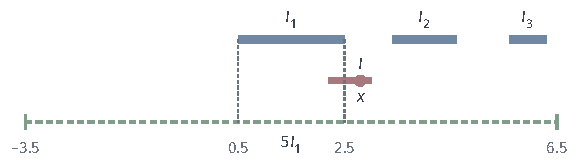
\includegraphics[width=97.991mm]{figures/04-spaces-measures-and-geometry/02-measure/tikz/integ-vitali-cover/figure.pdf}
  \caption{Vitali选择中的五倍放大。蓝色为已选的两两不交区间$I_1=[0.5,2.5]$、$I_2=[3.4,4.6]$、$I_3=[5.6,6.3]$；红色区间$I=[2.2,3.0]$含点$x$，与$I_1$相交且$\lvert I\rvert=0.8<2\lvert I_1\rvert$，因此落在与$I_1$同心、长为$10$的区间$5I_1=[-3.5,6.5]$（绿色虚线）中。}
  \label{fig:integ-vitali-cover}
\end{BookInlineFigure}

\paragraph{单调函数的导数}
为描述导数可能不存在的情况，对$x\in(a,b)$引入右侧差商$\bigl(F(x+h)-F(x)\bigr)/h$在$h\downarrow0$时的上极限$D^+F(x)$与下极限$D_+F(x)$，以及左侧差商$\bigl(F(x)-F(x-h)\bigr)/h$的上极限$D^-F(x)$与下极限$D_-F(x)$，统称\term{Dini导数}（Dini derivative）。$F$在$x$处可导当且仅当四者相等且有限。

下面的证明还要用到积分的平移不变性：对可积或非负可测的$\phi$与实数$h$，有
\[
 \int_{[a,b]}\phi(x+h)\,\mathrm dx=\int_{[a+h,b+h]}\phi(x)\,\mathrm dx .
\]
对指示函数这就是Lebesgue测度的平移不变性，由线性性推广到简单函数，再由递增逼近推广到非负可测函数和可积函数。

单调函数的增量总和被端点差控制，这个全局约束足以迫使差商在几乎每一点收敛。

\begin{theorem}[单调函数几乎处处可导]
\label{thm:integ-monotone-differentiable}
设$F:[a,b]\to\mathbb R$单调不减。则$F$在$[a,b]$上几乎处处有有限导数，$F'$（在导数不存在处取$0$）可积，并且
\begin{equation}
 \int_a^bF'(x)\,\mathrm dx\leq F(b)-F(a).
 \label{eq:integ-monotone-derivative-bound}
\end{equation}
\end{theorem}

\begin{proof}
先证四个Dini导数几乎处处相等。取有理数$0<u<v$，令
\[
 E=\{x\in(a,b):D_-F(x)<u<v<D^+F(x)\},\qquad s=\lambda^*(E).
\]
思路是用$E$上的两种差商夹出矛盾：左侧小区间上增量小于$u$倍长度，右侧小区间上增量大于$v$倍长度。

对$\varepsilon>0$取开集$O\supseteq E$，$\lambda(O)<s+\varepsilon$。每个$x\in E$都有任意小的$h>0$，使$[x-h,x]\subseteq O\cap(a,b)$且$F(x)-F(x-h)<uh$。这些区间构成$E$的Vitali覆盖，由引理~\ref{lem:integ-vitali}选出两两不交的$[x_k-h_k,x_k]$（$k\leq N$），未覆盖部分外测度小于$\varepsilon$，并且
\[
 \sum_k\bigl(F(x_k)-F(x_k-h_k)\bigr)<u\lambda(O)<u(s+\varepsilon).
\]

令$A$为$E$落在这些区间内部的部分，则$\lambda^*(A)>s-\varepsilon$。每个$y\in A$都有任意小的$k>0$，使$[y,y+k]$含于某个$(x_j-h_j,x_j)$且$F(y+k)-F(y)>vk$。再用引理选出两两不交的$J_1,\dots,J_M$，总长大于$s-2\varepsilon$，于是$F$在这些区间上的增量之和大于$v(s-2\varepsilon)$。

$F$单调不减，同一个$[x_k-h_k,x_k]$内不交子区间上的增量之和不超过它两端的增量。比较两次估计，得到
\[
 v(s-2\varepsilon)<u(s+\varepsilon).
\]
令$\varepsilon\to0$得$vs\leq us$。由$u<v$，只能$s=0$。

对所有有理数对取并，$D^+F\leq D_-F$几乎处处成立。把这一结论用于单调不减函数$\tilde F(x)=-F(-x)$，得到$D^-F\leq D_+F$几乎处处成立。于是几乎处处有
\[
 D^+F\leq D_-F\leq D^-F\leq D_+F\leq D^+F .
\]
四者相等，导数在$[0,+\infty]$中几乎处处存在。

再证积分估计，它同时说明导数几乎处处有限。对$x>b$令$F(x)=F(b)$，令$q_n(x)=n\bigl(F(x+1/n)-F(x)\bigr)$。单调函数的阈值集合是区间，所以$q_n$是非负可测函数，并在导数存在处$q_n\to F'$。由Fatou引理与平移不变性，
\[
\begin{aligned}
 \int_a^bF'\,\mathrm dx&\leq\liminf_n\int_a^bq_n\,\mathrm dx\\
 &=\liminf_n\Bigl(n\int_b^{b+1/n}F\,\mathrm dx-n\int_a^{a+1/n}F\,\mathrm dx\Bigr).
\end{aligned}
\]
在$[b,b+1/n]$上$F=F(b)$，在$[a,a+1/n]$上$F\geq F(a)$，所以右端不超过$F(b)-F(a)$。左侧有限，非负可积函数几乎处处有限。
\end{proof}

式~\eqref{eq:integ-monotone-derivative-bound}只是不等式。$[0,1]$上的阶跃函数$\mathbf 1_{[1/2,1]}$单调不减，除$x=1/2$外导数都是$0$，导数的积分为$0$，而端点增量为$1$；增量全部发生在一个点上，导数读不到它。所以单调性只给出导数的存在与总量的上界。

\paragraph{变上限积分的导数}
现在回到$G(x)=\int_a^xg$。证明思路是先得到$\int_a^c(G'-g)=0$对每个$c$成立，所以需要一个判零引理：区间上的积分全为零的函数几乎处处为零。

\begin{lemma}[区间积分全为零的函数]
\label{lem:integ-vanishing-intervals}
设$g$在$[a,b]$上可积且为实值。若对每个$x\in[a,b]$都有$\int_a^xg=0$，则$g=0$几乎处处成立。
\end{lemma}

\begin{proof}
Lebesgue可测函数与某个Borel函数几乎处处相等，改动零测集不影响结论，不妨设$g$是Borel函数。令$\mathcal D$为使$\int_Eg=0$的Borel集$E\subseteq[a,b]$全体。

区间$(c,d]\subseteq[a,b]$满足
\[
 \int_{(c,d]}g=\int_a^dg-\int_a^cg=0,
\]
这些区间与空集对有限交封闭，并生成$[a,b]$上的Borel集（单点零测，可以并入）。

$\mathcal D$是$\lambda$系统：$[a,b]\in\mathcal D$；补集由$\int_{E^c}g=\int g-\int_Eg$得到；两两不交的可数并由支配收敛（以$\lvert g\rvert$为控制）得到。由$\pi$--$\lambda$定理，$\mathcal D$包含全部Borel集。取$E=\{g>0\}$，得$\int g^+=0$，所以$g\leq0$几乎处处成立；同理$g\geq0$几乎处处成立。
\end{proof}

现在可以陈述本小节的主要结论。

\begin{theorem}[Lebesgue微分定理]
\label{thm:integ-lebesgue-differentiation}
设$g$在$[a,b]$上可积，$G$由式~\eqref{eq:integ-indefinite}给出。则$G$绝对连续，$G$几乎处处可导，并且$G'=g$几乎处处成立，即对几乎每个$x\in(a,b)$，
\begin{equation}
 \lim_{h\to0}\frac1h\int_x^{x+h}g(t)\,\mathrm dt=g(x).
 \label{eq:integ-lebesgue-differentiation}
\end{equation}
其中$h<0$时$\int_x^{x+h}$理解为$-\int_{x+h}^x$。
\end{theorem}

\begin{proof}
绝对连续性已经证明。复值情形对实部、虚部分别处理；实值情形由$g=g^+-g^-$与导数的线性性，只需对$g\geq0$证明。

先设$0\leq g\leq M$。此时$G$单调不减且是Lipschitz函数，由定理~\ref{thm:integ-monotone-differentiable}几乎处处可导。对$x>b$令$G(x)=G(b)$，差商$q_n(x)=n\bigl(G(x+1/n)-G(x)\bigr)$满足$0\leq q_n\leq M$，并在$G$可导处趋于$G'$。对$c\in(a,b]$，在$[a,c]$上以常数$M$为控制用支配收敛，再平移，得
\[
 \int_a^cG'\,\mathrm dx=\lim_{n\to\infty}\Bigl(n\int_c^{c+1/n}G\,\mathrm dx-n\int_a^{a+1/n}G\,\mathrm dx\Bigr).
\]
$G$连续，函数在缩小区间上的平均值趋于端点值，所以右端等于$G(c)-G(a)$。于是
\[
 \int_a^c(G'-g)\,\mathrm dx=0
\]
对所有$c$成立，由引理~\ref{lem:integ-vanishing-intervals}，$G'=g$几乎处处成立。

再看一般的$g\geq0$。令$g_n=\min\{g,n\}$，$G_n(x)=\int_a^xg_n$。由有界情形，$G_n'=g_n$几乎处处成立。函数$G-G_n=\int_a^x(g-g_n)$单调不减，其导数几乎处处非负，所以$G'\geq g_n$几乎处处成立；合并可数个例外集，得$G'\geq g$几乎处处成立。

另一方面，由式~\eqref{eq:integ-monotone-derivative-bound}，
\[
 \int_a^bG'\,\mathrm dx\leq G(b)-G(a)=\int_a^bg\,\mathrm dx .
\]
因此$G'-g\geq0$几乎处处成立且积分不超过$0$，由定理~\ref{thm:integ-monotonicity}，$G'=g$几乎处处成立。
\end{proof}

定理的名称来自式~\eqref{eq:integ-lebesgue-differentiation}：$g$在$x$附近的局部平均值，在几乎每一点恢复$g$的取值。卷一要求$g$连续，结论在每一点成立；这里$g$只是可积，结论在零测集外成立。

下面用一个能手算的例子看例外集。在$[0,2]$上取$g=\mathbf 1_{[0,1]}$，变上限积分是
\[
 G(x)=\min\{x,1\}.
\]
除$x=1$外$G$都可导，$x<1$时$G'=1=g$，$x>1$时$G'=0=g$；在$x=1$处$G$有折角，导数不存在。例外集是单点，与定理相符。

$[0,1]$上的$\mathbf 1_{\mathbb Q}$说明“几乎处处”不能改成“处处”：它的变上限积分恒为$0$，导数$0$与$\mathbf 1_{\mathbb Q}$在每个有理点都不同。

\subsection{由导数恢复函数}
\label{sec:integ-recovery}

\paragraph{有界变差与导数的存在}
现在处理第二个方向：给定绝对连续的$F$，要证明$F(x)=F(a)+\int_a^xF'$。第一步是确认$F'$几乎处处存在且可积。对$[a,b]$的分割$P:a=x_0<\dots<x_n=b$，令
\[
 V(F,P)=\sum_k\lvert F(x_k)-F(x_{k-1})\rvert .
\]
称$V_a^b(F)=\sup_PV(F,P)$为$F$在$[a,b]$上的变差，它是函数图像沿纵向走过的总路程；若它有限，称$F$为\term{有界变差函数}（function of bounded variation）。在分割中插入点只会使$V(F,P)$不减，所以变差对区间可加：$V_a^b(F)=V_a^c(F)+V_c^b(F)$。

\begin{lemma}[绝对连续函数有界变差]
\label{lem:integ-ac-bv}
若$F$在$[a,b]$上绝对连续，则$F$是有界变差函数，并且是两个单调不减函数之差。
\end{lemma}

\begin{proof}
对$\varepsilon=1$取定义中的$\delta$，把$[a,b]$等分成$K$段，每段长度小于$\delta$。在一段$[c,d]$内任取分割，其小区间两两不交、总长小于$\delta$，增量之和小于$1$，故$V_c^d(F)\leq1$。由区间可加性，$V_a^b(F)\leq K$。

令$V(x)=V_a^x(F)$。对$x<y$，$V(y)-V(x)=V_x^y(F)\geq\lvert F(y)-F(x)\rvert$，所以$V$与$V-F$都单调不减，而$F=V-(V-F)$。
\end{proof}

由定理~\ref{thm:integ-monotone-differentiable}，两个单调函数都几乎处处可导且导数可积，所以绝对连续函数$F$几乎处处可导，$F'$可积。

\paragraph{零导数引理}
令$H(x)=F(x)-F(a)-\int_a^xF'$。由上一小节，$H$绝对连续且$H'=F'-F'=0$几乎处处成立。恢复公式就归结为：导数几乎处处为零的绝对连续函数必为常数。阶跃函数说明没有绝对连续性时这不成立；绝对连续性的作用，是控制导数为零的点之外那些总长很小的间隙上的增量。

\begin{lemma}[零导数引理]
\label{lem:integ-zero-derivative}
若$H$在$[a,b]$上绝对连续，且$H'=0$几乎处处成立，则$H$是常数。
\end{lemma}

\begin{proof}
任取$c\in(a,b]$，证明$H(c)=H(a)$。给定$\varepsilon>0$，取绝对连续定义中的$\delta$。令$E=\{x\in(a,c):H'(x)=0\}$，则$\lambda(E)=c-a$。

对每个$x\in E$，有任意小的$h>0$使$[x,x+h]\subseteq(a,c)$且$\lvert H(x+h)-H(x)\rvert<\varepsilon h$。这些区间构成$E$的Vitali覆盖，由引理~\ref{lem:integ-vitali}选出两两不交的$[x_k,y_k]$（$k=1,\dots,N$，按$x_1<y_1<x_2<\dots<y_N$排列），使$\lambda\bigl(E\setminus\bigcup_k[x_k,y_k]\bigr)<\delta$。

记$y_0=a$、$x_{N+1}=c$。剩下的间隙$(y_k,x_{k+1})$两两不交，总长小于$\delta$。把端点增量沿选中区间和间隙拆开：
\[
 \lvert H(c)-H(a)\rvert\leq\sum_{k=1}^N\lvert H(y_k)-H(x_k)\rvert+\sum_{k=0}^N\lvert H(x_{k+1})-H(y_k)\rvert .
\]
第一个和由导数为零控制，不超过$\varepsilon\sum_k(y_k-x_k)\leq\varepsilon(c-a)$；第二个和由绝对连续性控制，小于$\varepsilon$。于是
\[
 \lvert H(c)-H(a)\rvert<\varepsilon(c-a)+\varepsilon .
\]
$\varepsilon$任意，所以$H(c)=H(a)$。
\end{proof}

\paragraph{恢复公式}
零导数引理补上了最后一步，两个方向合起来给出一个双向刻画。

\begin{theorem}[Lebesgue微积分基本定理]
\label{thm:integ-ftc}
设$F:[a,b]\to\mathbb R$。以下两条等价：
\begin{enumerate}
 \item $F$在$[a,b]$上绝对连续；
 \item 存在$[a,b]$上的可积函数$g$，使$F(x)=F(a)+\int_a^xg(t)\,\mathrm dt$对所有$x\in[a,b]$成立。
\end{enumerate}
此时$F$几乎处处可导，$F'=g$几乎处处成立，并且对任意$c,x\in[a,b]$，
\begin{equation}
 F(x)=F(c)+\int_c^xF'(t)\,\mathrm dt,
 \label{eq:integ-ftc}
\end{equation}
其中$x<c$时$\int_c^x$理解为$-\int_x^c$。
\end{theorem}

\begin{proof}
(2)推出(1)及$F'=g$几乎处处成立，就是定理~\ref{thm:integ-lebesgue-differentiation}。

(1)推出(2)。由引理~\ref{lem:integ-ac-bv}，$F'$几乎处处存在且可积。令$H(x)=F(x)-F(a)-\int_a^xF'$，它绝对连续且$H'=0$几乎处处成立。由引理~\ref{lem:integ-zero-derivative}，$H\equiv H(a)=0$，取$g=F'$即得(2)。

式~\eqref{eq:integ-ftc}由$x$与$c$两处的(2)相减得到。
\end{proof}

这一形式的\term{微积分基本定理}（fundamental theorem of calculus）说：绝对连续函数恰好是可积函数的变上限积分加上常数，这个可积函数在几乎处处的意义下唯一确定为$F'$。

式~\eqref{eq:integ-ftc}说明怎样恢复整个函数：只需知道一点的函数值$F(c)$和一个可积的导数代表。导数在零测集上的取值无关紧要，函数值却要在一点给定，否则只能恢复到相差一个常数。

例如$F(x)=\lvert x\rvert$在$[-1,1]$上是Lipschitz函数，因而绝对连续。除$x=0$外$F'(x)=\operatorname{sgn}x$。从$c=-1$出发恢复，
\[
 F(0)=F(-1)+\int_{-1}^0(-1)\,\mathrm dt=1-1=0,
\]
再继续恢复到右端点，
\[
 F(1)=F(0)+\int_0^11\,\mathrm dt=1 .
\]
两个值都与$\lvert x\rvert$一致；$F'$在$x=0$处没有定义，并不影响恢复。

\paragraph{Cantor函数}
仅有连续性和几乎处处可导，还不能保证恢复公式。下面用Cantor集构造一个反例。记第~\ref{chap:measure}章Cantor集构造中第$n$步的$2^n$个保留闭区间之并为$C_n$。令$c_n:[0,1]\to[0,1]$是这样的连续分段线性函数：$c_n(0)=0$，在$C_n$的每个保留区间上线性增加$2^{-n}$，在已删去的开区间上取常值，于是$c_n(1)=1$。

从$c_n$到$c_{n+1}$，在每个保留区间上，原来线性增加的$2^{-n}$被分成左、右三分之一上各增加$2^{-n-1}$，中间三分之一上不变；两端的值不变。在同一个保留区间上，$c_n$与$c_{n+1}$都是单调函数，从相同的起点走到相同的终点，总上升量是$2^{-n}$，所以二者之差不超过$2^{-n}$。在已删去的区间上二者相等。于是
\[
 \sup_{[0,1]}\lvert c_{n+1}-c_n\rvert\leq2^{-n}.
\]
所以$c_n$一致收敛到一个连续函数$c$，称为\term{Cantor函数}（Cantor function）。它单调不减，$c(0)=0$，$c(1)=1$，并且在每个删去的开区间上取常值，因为从删去这一区间的那一步起，所有$c_n$在其上都取同一个常值。图~\ref{fig:integ-cantor-function}画出了前几步的逼近。

\begin{BookInlineFigure}
  \centering
  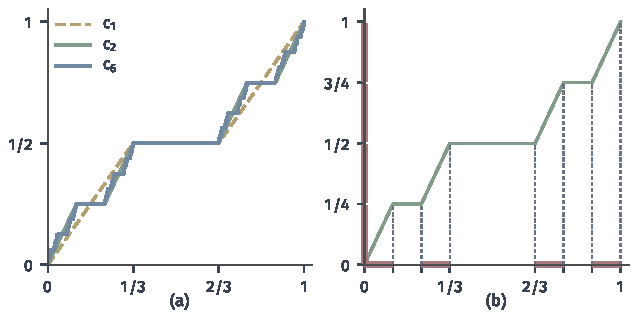
\includegraphics[width=108mm]{figures/04-spaces-measures-and-geometry/02-measure/matplotlib/integ-cantor-function/figure.pdf}
  \caption{Cantor函数及其分段线性逼近。(a)$c_1$（黄色虚线）、$c_2$（绿）与$c_6$（蓝），$c_n$在第$n$步的$2^n$个保留区间上线性增加$2^{-n}$，在已删去的区间上保持常值。(b)第二步的四个保留区间$[0,\frac19]$、$[\frac29,\frac13]$、$[\frac23,\frac79]$、$[\frac89,1]$（横轴红色）总长$\frac49$，对应的增量（纵轴红色）各为$\frac14$，合起来覆盖整个$[0,1]$。}
  \label{fig:integ-cantor-function}
\end{BookInlineFigure}

$[0,1]\setminus C$是删去的开区间之并，$c$在其中每一点导数为$0$；$\lambda(C)=0$，所以$c'=0$几乎处处成立，而
\[
 \int_0^1c'(x)\,\mathrm dx=0\neq1=c(1)-c(0).
\]
恢复公式失败，由定理~\ref{thm:integ-ftc}，$c$不绝对连续。这也可以直接从定义看出：第$n$步的$2^n$个保留区间（取其内部）两两不交，总长$(2/3)^n\to0$，$c$在它们上的增量之和始终是$1$。

Cantor函数把几种容易混淆的性质分开了。它连续，所以连续不能保证恢复公式；它单调，因而有界变差并且几乎处处可导，所以这两条也不够；它缺的正是绝对连续性。在$[a,b]$上有
\begin{equation}
 \text{Lipschitz}\Rightarrow\text{绝对连续}\Rightarrow\text{连续且有界变差}\Rightarrow\text{几乎处处可导},
 \label{eq:integ-regularity-chain}
\end{equation}
三个箭头都不能反过来，反例依次是$\sqrt x$、Cantor函数与阶跃函数$\mathbf 1_{[1/2,1]}$。

Cantor函数作为Stieltjes测度的累积函数，给出一个没有点质量、却集中在零测集$C$上的概率测度；第~\ref{chap:measure-densities}章把实轴上的测度分解为点质量、绝对连续与这类奇异连续三部分时，它是奇异连续部分的标准例子。
